\chapter{Example Model of Packet Processing System}
\label{chapter:example-simulation-model}

In this chapter, we present an example of how to model a network processing system. The example model is built based on a Cavium OCTEON II hardware. We will first demonstrate the measurement setup needed to obtain the reference values for the model. Two different measurements will be done, one to measure the communication latencies and another to measure the memory latencies. After that, we will plug in the reference values to the model and describe the relevant details of it.

\section{Reference Values}
\label{sec:reference-values}

\fixme{TODO} Reference values are used to tune the model so that the simulation behavior corresponds with execution of the real system. The parameters should at the same time be precise - the simulation should bring out the desired system behavior with accurate precision, and abstract - the simulation model by definition should be an abstraction of the modeled system. The decision between the level of accuracy and abstraction usually requires knowledge of the system under modeling.

The following subchapters describe the implemented setup used to measure values for the simulation model. First, we will present the hardware used for the measurements, and discuss the decisions for our parameter selection. After that we will demonstrate how the measurements were done.

% For our approach to be valid, i.e. the abstraction of the communication latencies to be precise enough, we have to assume the fastpath is not the bottleneck in the processing phase. This assumption is reasonable because ...

% \fixme{
%   TODO:
%   \begin{itemize}
%   \item because the fastpath hardware is optimized for this task
%   \item find reference
%   \item maybe justify the stuff with some kind of rough back-of-the-envelope calculation?
%   \end{itemize}
% }

\subsection{Measurement Hardware}
\fixme{
  \begin{itemize}
  \item Example of relevant fastpath hardware
  \item NOT an example of balanced distributed (virtualized) fastpath system
  \item but helps us figure out the relevant values of fastpath system needed for the model
  \end{itemize}
}

\subsection{Communication Latencies}

We measured the communication latencies of the example fastpath by generating traffic from external machine, and sending it through two OCTEON II blades back to the generator. We did the measurements at two independent points in the processing path, to validate the accuracy of the measurements.

\begin{figure}[ht]
  \begin{center}
    \tikzstyle{block} = [draw, rectangle, thick, minimum height=2em, minimum width=2em]
\tikzstyle{dot} = [circle, inner sep=0pt, minimum size=1mm, fill=black,draw=black]
\tikzstyle{connector} = [->, thick]
\tikzstyle{line} = [thick]

\begin{tikzpicture}
  \small
  % node placement with matrix library: 5x4 array
  \matrix[ampersand replacement=\&, row sep=0.2cm, column sep=0.4cm] {
    \node[block] (l1) {External Traffic-Generator}; \& \& \&
    \node[block] (c1) {Forward Blade}; \& \& \&
    \node[block] (r1) {Swap Blade}; \& \\
  };

  %% Traffic gen probes
  \node [dot] (ld1) at ($(l1.10) + (0cm, 0.4cm)$) {};
  \draw [line] (l1.10) -- node[] {} (ld1);

  \node [dot] (ld2) at ($(l1.-10) + (0cm, -0.4cm)$) {};
  \draw [line] (l1.-10) -- node[] {} (ld2);

  %% Forward blade probes
  \node [dot] (cd1) at ($(c1.18) + (0cm, 0.4cm)$) {};
  \draw [line] (c1.18) -- node[] {} (cd1);

  \node [dot] (cd2) at ($(c1.-18) + (0cm, -0.4cm)$) {};
  \draw [line] (c1.-18) -- node[] {} (cd2);

  %% Swap blade probes
  \node [dot] (rd1) at ($(r1.157) + (0cm, 0.4cm)$) {};
  \draw [line] (r1.157) -- node[] {} (rd1);

  \node [dot] (rd2) at ($(r1.-157) + (0cm, -0.4cm)$) {};
  \draw [line] (r1.-157) -- node[] {} (rd2);

  %% Arrows connecting the nodes

  \draw [connector] (l1.7) -- node[] {} (c1.168);
  \draw [connector] (c1.12) -- node[] {} (r1.166);
  \draw [connector] (r1.-166) -- node[] {} (c1.-12);
  \draw [connector] (c1.-168) -- node[] {} (l1.-7);

\end{tikzpicture}

%%% Local Variables:
%%% mode: latex
%%% TeX-master: "../thesis-hartikainen.tex"
%%% End:

    \caption{The setup used to measure the communication latencies. The measurement points shown with the probes. \fixme{TODO: Make this figure clearer, Emphasize the input and output parts of the flow.}}
    \label{fig:comm-setup}
  \end{center}
\end{figure}

In figure~\ref{fig:comm-setup}, the rectangles represent three different computing units (traffic generator, forward blade, and swap blade), and the probes present the points of time measurements. The traffic generator used is a typical desktop computer running Linux and the traffic was generated by Mausezahn \fixme{reference}. Both of the OCTEON II blades are running Linux.

The packet is first generated at the packet generator and sent to the forward blade at time $t_{d0}$. Forwarding blade receives the packet, does the needed processing and forwards the packet to the swap blade at time $t_{d1}$. The swap blade receives the packet at time $t_{r2}$, does the same processing as the forward blade (except with different destination address), and forwards the packet back to the forward blade at time $t_{d2}$. Finally the forward blade receives the packet at time $t_{r1}$ and forwards it to the traffic generator, which marks it received at time $t_{r0}$.

We measured the times for packet sizes of 64B, 128B, 256B, 512B, 1024B, and 1500B, repeating the measurement for each packet 10000 times. The time $t_{f}$ spent in the fastpath (input and output) phase of one blade is then

\begin{equation}
  \label{eq:1}
  t_{f} = \frac{t_{r1} - t_{d1} - (t_{d2} - t_{r2})}{2}
\end{equation}

Figure~\ref{fig:comm-latency} shows the resulting times $t_{f}$ for the different packet sizes.

\begin{figure}[h]
  \begin{center}
    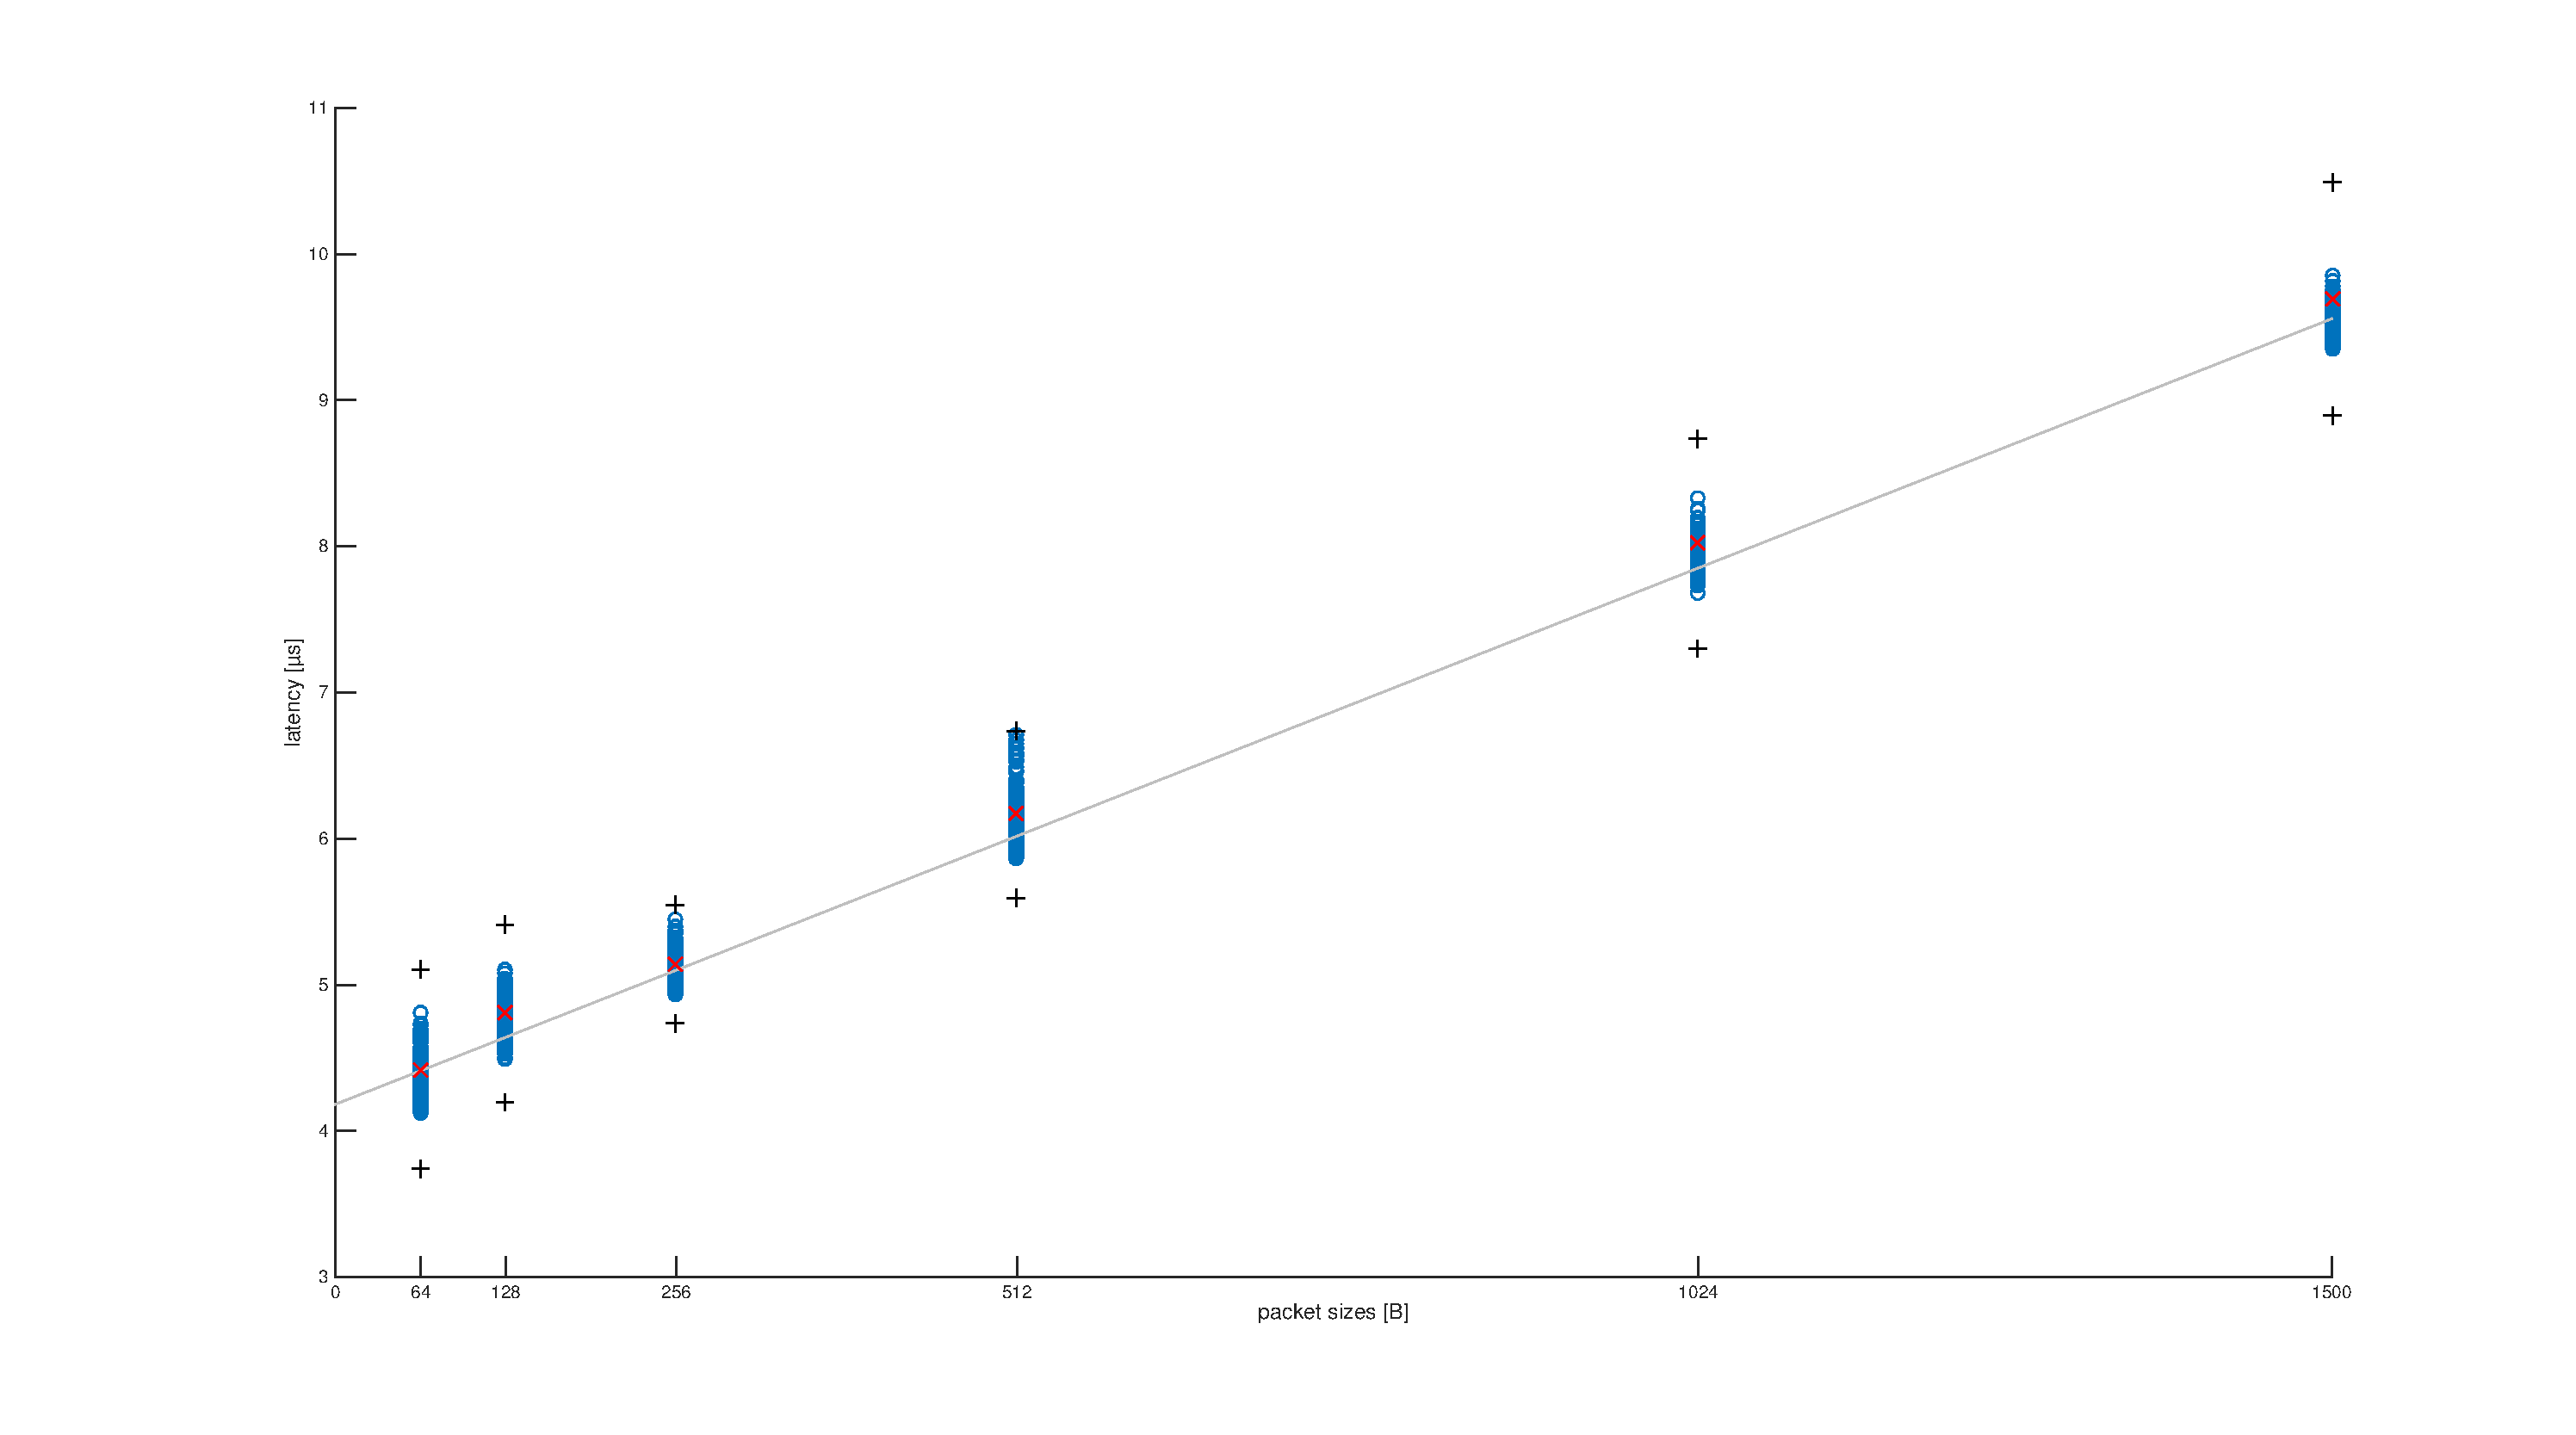
\includegraphics[width=\textwidth]{images/comm-latency.pdf}
    \caption{Latency of the fastpath (input and output) phase of the OCTEON II board. Averages shown marked as red x, and the 99\% \fixme{check the confint} confidence intervals with +. The trendline is of equation \fixme{latency = a*packetsize + constant}.}
    \label{fig:comm-latency}
  \end{center}
\end{figure}

As figure ~\ref{fig:comm-latency} shows us, the time spent in the input and output phase of the board is linear regarding to the packet size. The variation of the data is relatively small, and all the measurements correspond to the values measured with the external traffic-generator.

\fixme{
  TODO: the following needs to be explained somewhere with the other fastpath stuff.
  \begin{enumerate}
  \item Regardless of the packet size, the size of the work queue entry handled by the input/output units is the same.
  \item Also, the forward/swap code is constant in terms of packet size.
  \item Only operation that is dependent on the packet size is the copy from input to L2/RAM and from L2/RAM to output unit.
  \end{enumerate}
}

As explained earlier \fixme{explain this}, the only packet size dependent operations in the fastpath are the  memory transfers between the memory (L2/RAM) and PKI or PKO.

\subsection{Memory Delays}

Memory delays were measured using Multi-core Processor Architecture and Communication (MPAC) benchmarking library. \ref{referenssi} Both, latency and throughput, were measured using for different dataset sizes and number of threads.

\begin{figure}[h]
  \begin{center}
    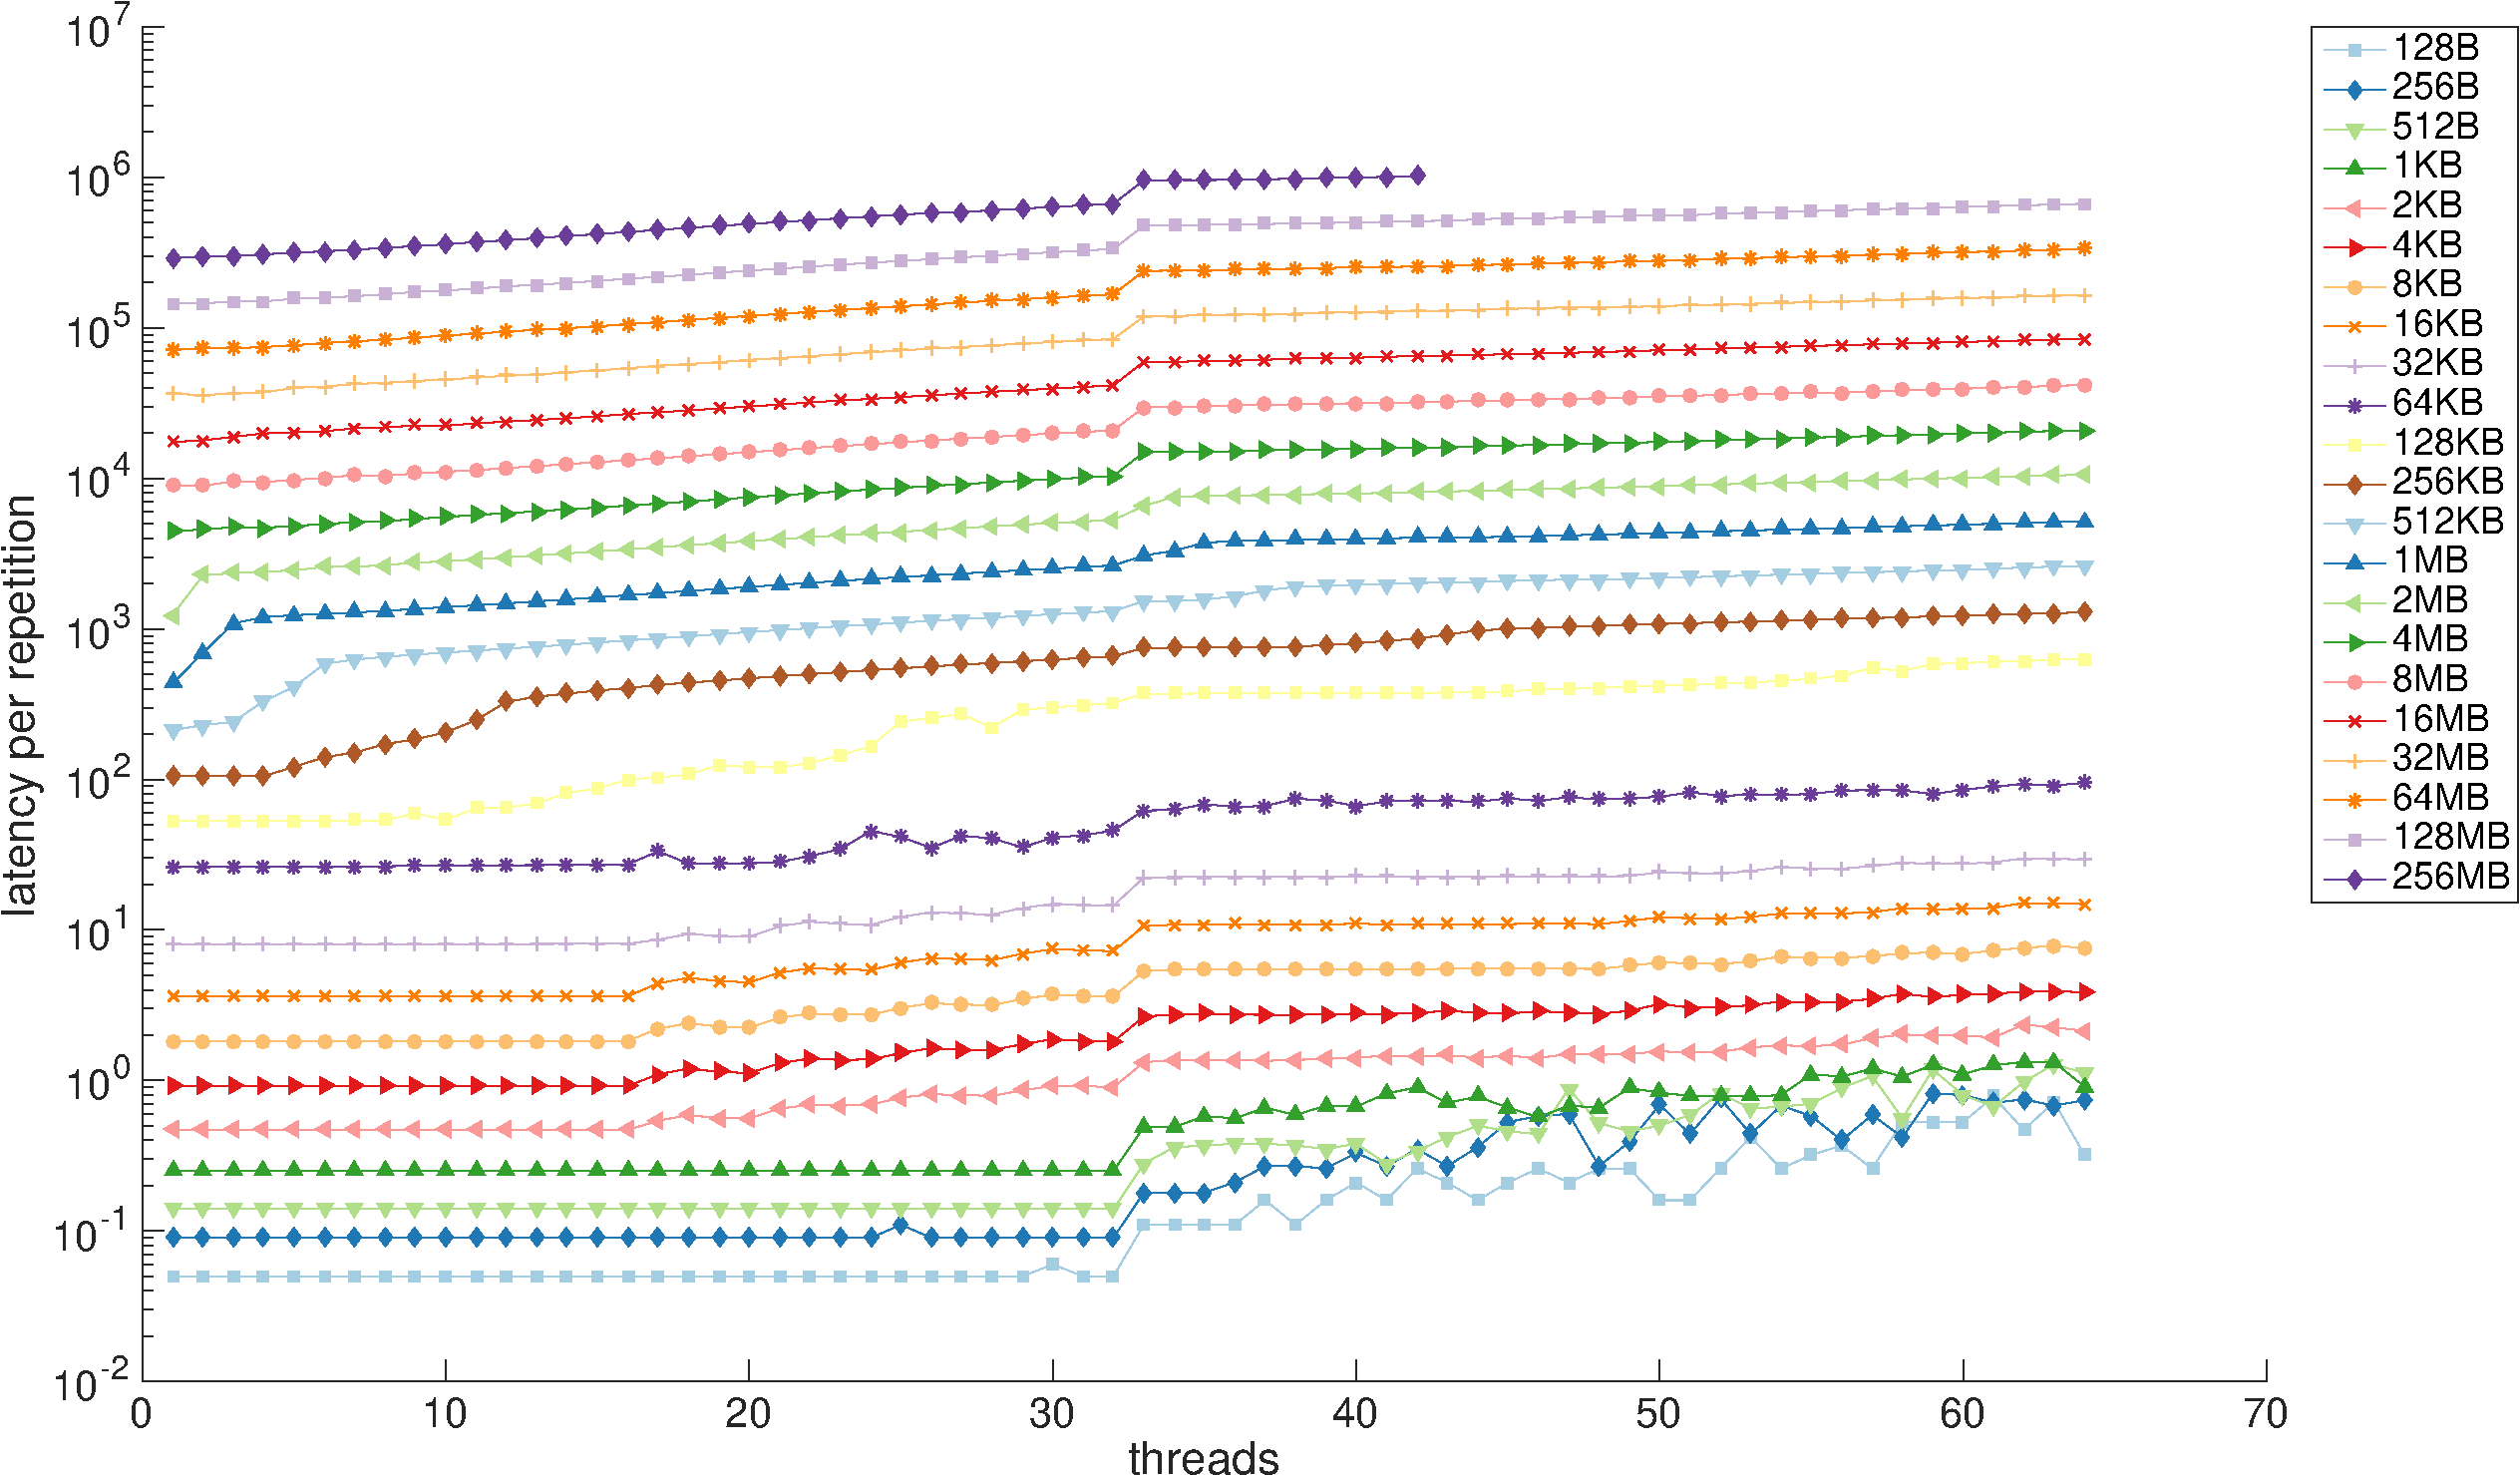
\includegraphics[width=\textwidth]{images/mem-latency.pdf}
    \caption{Memory latencies of the example NPU, measure by MPAC. \fixme{logarithmic Y-scale}}
    \label{fig:mem-latency}
  \end{center}
\end{figure}

\begin{figure}[h]
  \begin{center}
    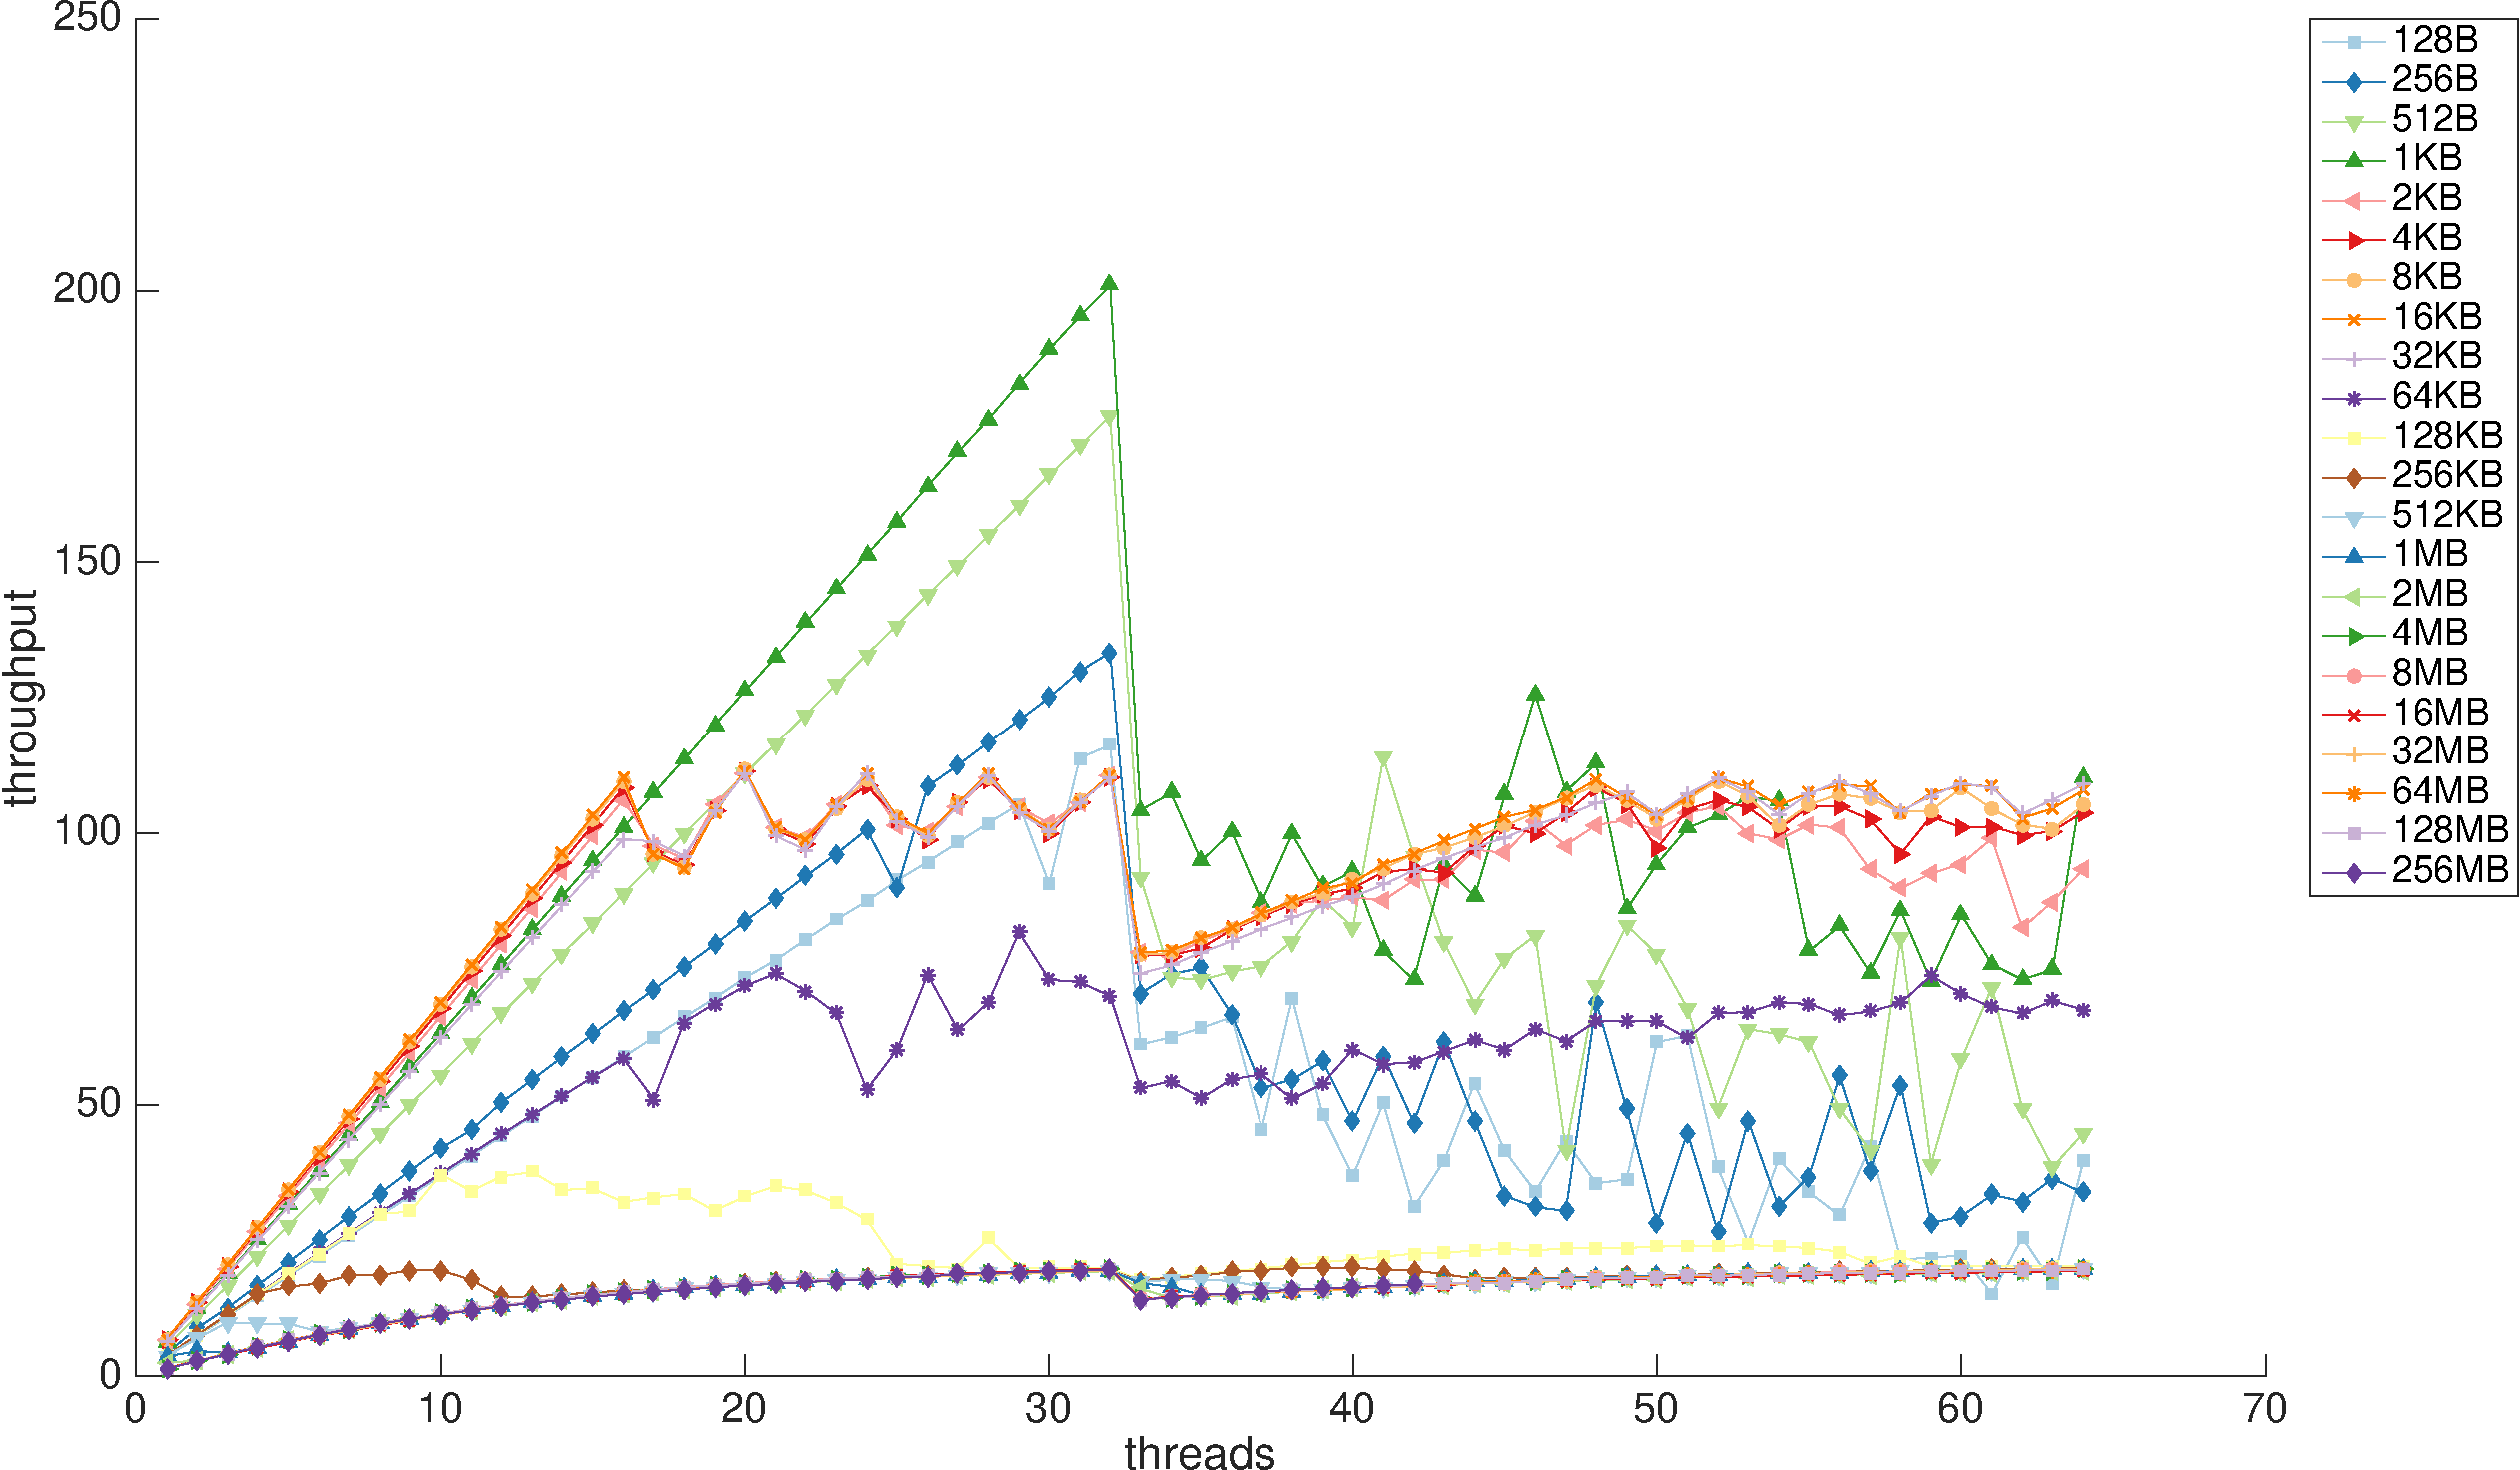
\includegraphics[width=\textwidth]{images/mem-throughput.pdf}
    \caption{Memory throughput of the example NPU, measure by MPAC.}
    \label{fig:mem-throughput}
  \end{center}
\end{figure}

As in the

\section{Workload Model}
\fixme{
  TODO: workload
}


\section{Hardware Model}
\fixme{
  Scheduler, input/output, NPU nodes
}

\section{Software Model}
\fixme{
  Scheduler, OpenEM-type application model
}

%%% Local Variables:
%%% mode: latex
%%% TeX-master: "thesis-hartikainen"
%%% End:
